\documentclass[11pt,dvipsnames]{beamer}
\usetheme{default} 

\setbeamertemplate{navigation symbols}{} %gets rid of navigation symbols
\setbeamertemplate{footline}{} %gets rid of bottom navigation bars
\setbeamertemplate{footline}[page number]{} %use this for page numbers

\setbeamertemplate{footline}{%
  \raisebox{5pt}{\makebox[\paperwidth]{\hfill\makebox[10pt]{\scriptsize\insertframenumber~~}}}}

\setbeamertemplate{itemize items}[circle] %round bullet points
\setlength\parskip{10pt} % white space between paragraphs

\usepackage{wrapfig}
\usepackage{subfig}
\usepackage{setspace}
\usepackage{enumerate}
\usepackage{graphicx}
\usepackage{amsmath}
\usepackage{amsfonts}
\usepackage{amssymb}
\usepackage{amsthm}
\usepackage[UKenglish]{isodate}
\usepackage{tikz}
\usepackage{pgfplots}
\usepackage{natbib}
\usepackage{hyperref}
\hypersetup{
    colorlinks=true, 
    urlcolor=blue
}
\def\checkmark{\tikz\fill[scale=0.4](0,.35) -- (.25,0) -- (1,.7) -- (.25,.15) -- cycle;} 

% allow drawing arrows
\usetikzlibrary{arrows}
\tikzstyle{arrow}=[draw, -latex] 

% bracketing shortcuts
\newcommand{\paren}[1]{\left(#1\right)}
\newcommand{\sqbracket}[1]{\left[#1\right]}
\newcommand{\cbracket}[1]{\left\{#1\right\}}
\newcommand{\abs}[1]{\left\lvert#1\right\rvert}
\newcommand{\norm}[1]{\left\lVert#1\right\rVert}
% set up the argmin operator, argmax
\DeclareMathOperator*{\argmin}{arg\,min}
\DeclareMathOperator*{\argmax}{arg\,max}

\newcommand{\myframe}[1]{\begin{frame} \frametitle{#1}}

% New itemize environment, with spaces
\newenvironment{spaceitemize}
{ \begin{itemize}
    \setlength{\itemsep}{10pt}
    \setlength{\parskip}{0pt}
    \setlength{\parsep}{0pt}     }
{ \end{itemize}                  } 


% the preamble
\title{Day 3, Session 1: R and RStudio basics}
\author{Jessica Williams-Nguyen and Brian D. Williamson}
\institute{EPI/BIOST Bootcamp 2018}
\date{25 September 2018}

% Start the document
\begin{document}
% The title page
\begin{frame}
\titlepage
\end{frame}

\begin{frame}
\frametitle{Learning objectives}
By the end of this session, you should be able to
\begin{itemize}
\item \textbf{organize} your files for a data analysis
\item \textbf{download} data from the internet
\item \textbf{load} data into an R workspace
\item \textbf{explore} your data (subset, index, plot, summarize) 
\item \textbf{load} R packages
\end{itemize}
\end{frame}

\begin{frame}
\frametitle{Goals}
R and RStudio are \textcolor{blue}{powerful} tools that make analyzing data and doing reproducible research easier (in the long run). 

However, before you become familiar with these tools, they may be frustrating to use.

\pause
This module is meant to give you a space to engage with R and RStudio prior to diving into coursework. \textbf{All R functions required for your courses will be introduced in the specific course}.
\end{frame}

\section{Organizing your workspace}
\begin{frame}
\frametitle{Organization: helping future you}
The first step in a data analysis isn't opening R or RStudio -- instead, you should create a \textcolor{blue}{workspace} for your analysis. \pause

This workspace is a \textbf{folder} on your computer that: \vspace{-0.3cm}\pause
\begin{itemize}
\item is \textcolor{ForestGreen}{easy for you to find \textbf{now}} \pause
\item will be \textcolor{cyan}{easy for you to find in the \textbf{future}} \pause
\item will hold \textbf{all relevant files} for your analysis (e.g., the data file, R code, plots, results)
\end{itemize}
\end{frame}

\begin{frame}
\frametitle{Organization: developing your workflow}
It is important that you develop your own workflow, since \textit{easy to find} means different things to everyone.

My workflow looks something like this: \vspace{-0.3cm} \pause
\begin{enumerate}
\item get involved in a new project \pause
\item set up a new folder for the project 
\begin{itemize}
\item under \textit{Courses} if it relates to a course, e.g., \texttt{Courses/BIOST511}
\item under \textit{the name of the project} if not, e.g., \texttt{Projects/HPTN063} refers to a clinical trial I have worked on
\end{itemize} \pause
\item store all documents, data, code, and output in this folder (with subfolders for each of these)
\end{enumerate}
\end{frame}

\begin{frame}
\frametitle{Downloading data}
The datasets for your coursework will typically be found either \vspace{-0.3cm}
\begin{itemize}
\item on \textbf{Canvas}, the UW's file-hosting site for courses, or
\item on \textcolor{ForestGreen}{your professor's webpage}, or
\item on the \textcolor{cyan}{webpage for a textbook}
\end{itemize}

Your instructor will tell you \textbf{exactly where} to find the datasets necessary for your coursework.

Once you have set up a folder (workspace) for your project, download the data into this folder.
\end{frame}

\begin{frame}
\frametitle{Exercise: downloading data}
Create a new folder titled \texttt{fev\_analysis} in the folder you are using for the files for this workshop.

Next, go to the Canvas webpage for this workshop and download the file \texttt{fev.txt}, located in the \texttt{Data} folder under the \texttt{Files} tab. Download these data into the \texttt{fev\_analysis} folder.
\end{frame}

% R intro
\section{The R and RStudio interfaces}
\begin{frame}
\frametitle{Using R and RStudio}
Once you have set up a workspace on your computer for your new project, and downloaded your data, it's time to use R! \pause

R is a \textcolor{blue}{statistical programming language}, and does all of the computing for your analysis (e.g., plots, summaries). 

RStudio is a \textcolor{ForestGreen}{program} that makes it easier to interact with R to perform your analysis. \pause

I suggest that you \textbf{only interact with R through RStudio} -- this is all you need for your Biostatistics coursework.
\end{frame}

\myframe{Using R and RStudio: the interface}
We interact with both R and RStudio using an interface. For R, this is the command line. For RStudio, this is the graphical user interface.

Both of these concepts deserve a bit of introduction, since familiarity with the interface makes using R and RStudio much easier!
\end{frame}

\myframe{Using R and RStudio: RStudio}
When you first open RStudio, you are met with a blank set of four \textcolor{blue}{panes}:
\begin{center}
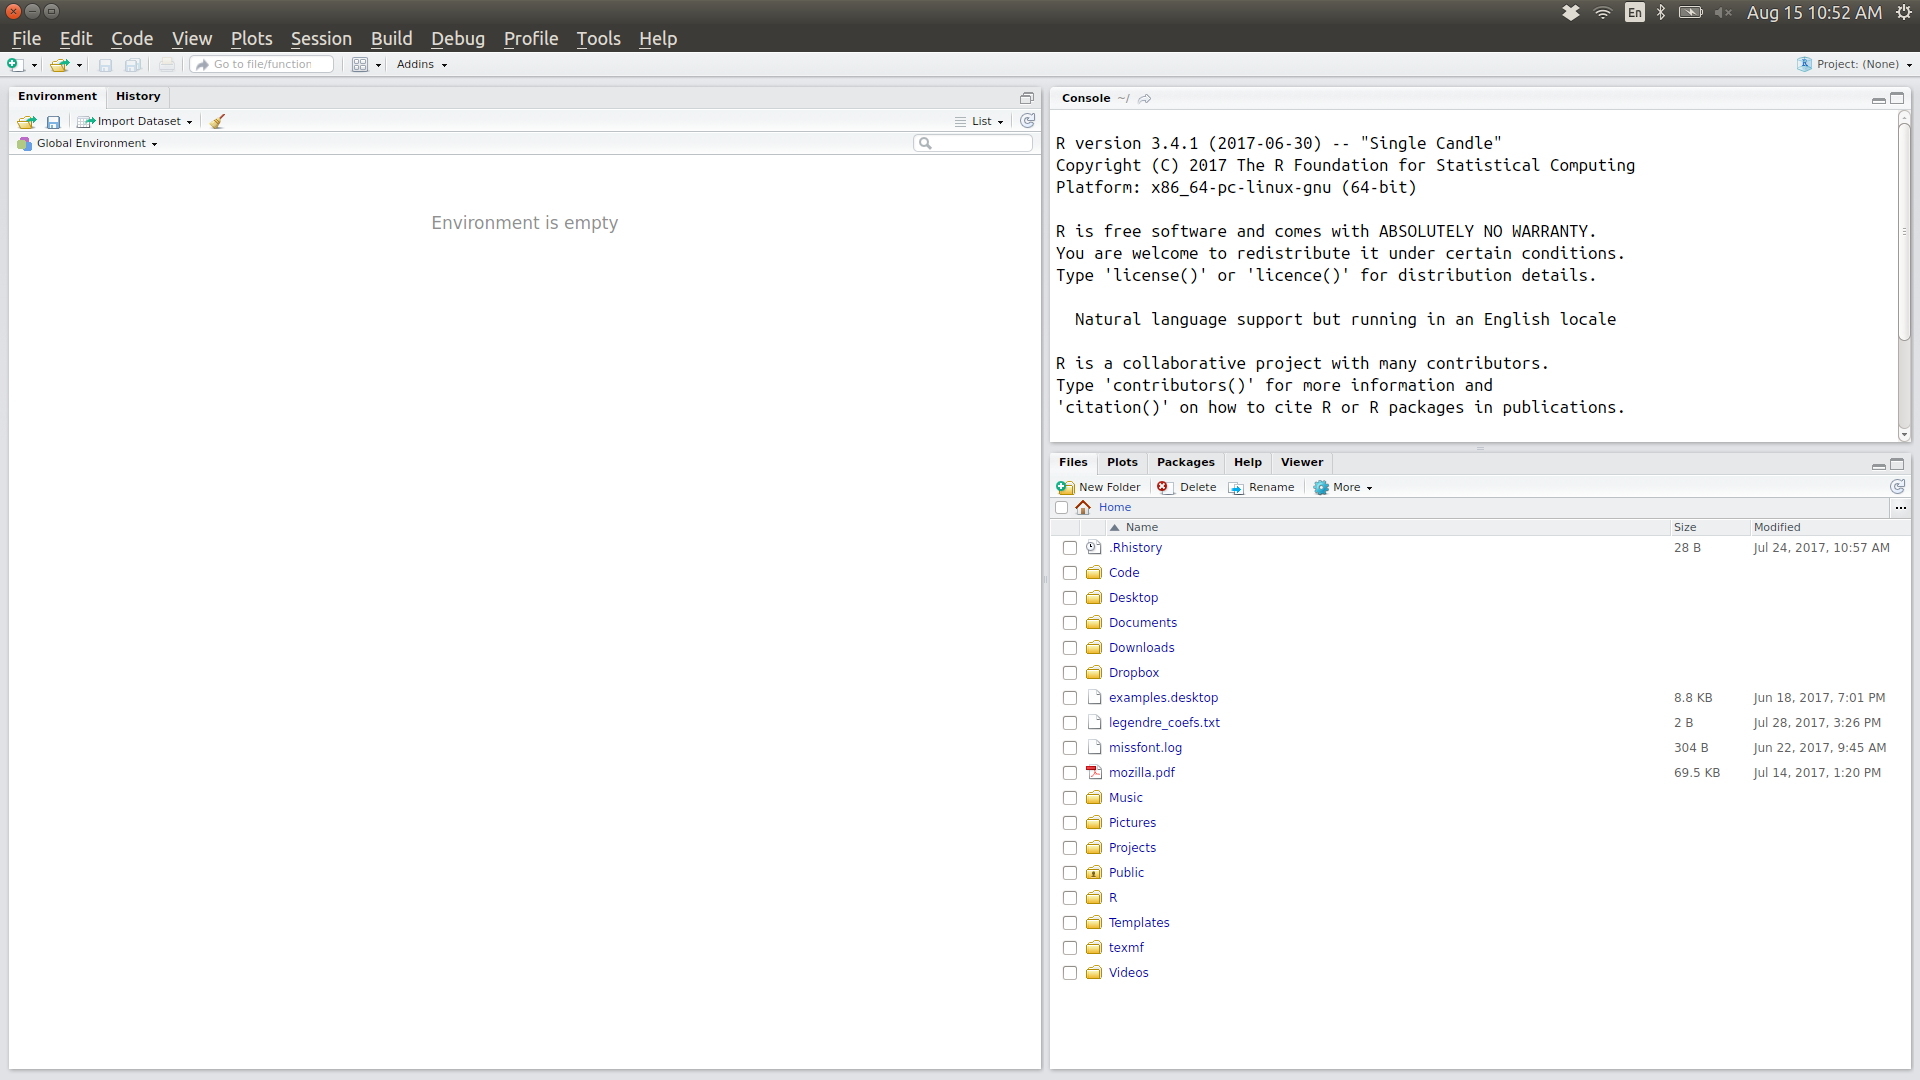
\includegraphics[width = 0.8\textwidth]{figs/rstudio.png}
\end{center}
\end{frame}

\myframe{Using R and RStudio: RStudio}
You can edit pane layout under \texttt{Tools > Global Options > Pane Layout}. My preference is to have the \textcolor{blue}{source} in the upper left, \textcolor{green}{console} in the upper right, \textcolor{cyan}{environment} in the lower left, and \textcolor{purple}{viewer} in the lower right.

You'll notice that on the previous slide, there were only three panes visible: since we haven't opened or created any files to edit, the \textcolor{blue}{source} pane is not currently open.
\end{frame}

\subsubsection{The console}
\myframe{RStudio: the console}
The \textcolor{green}{console} is our interface to the R command line. 

Any commands that we wish to enter go through the console, and any results that are output by these commands will appear in the console. 

\end{frame}

\begin{frame}[fragile]
\frametitle{Example: the console}
Typing \texttt{47} at the \texttt{>} symbol (from now on, called the execution line) and hitting \texttt{Enter} on the keyboard yields the following:
\begin{verbatim}
> 47
[1] 47
\end{verbatim}
\pause
Since R is a \textcolor{blue}{functional} programming language, typing \texttt{47} and hitting \texttt{Enter} is the same thing as using the \texttt{print()} function:
\begin{verbatim}
> print(47)
[1] 47
\end{verbatim}
\pause
The output is displayed as a \textcolor{green}{vector}, one of the fundamental \textcolor{cyan}{data structures} in R. The \texttt{[1]} helps to tell which element of the vector we are looking at (which is most useful if the vector spans multiple lines in the console).
\end{frame}

\begin{frame}
\frametitle{Exercise: the console}
Use the RStudio console to perform the following computations. Write down your answers and your process for arriving at your answers.
\begin{enumerate}
\item Multiply 55 and 389
\item Divide 500 by 15
\item Add 1525 and 3225
\end{enumerate}
\end{frame}

\begin{frame}
\frametitle{Exercise: the console}
You just used your first R functions! 

The \texttt{*}, \texttt{+} and \texttt{-}, and \texttt{/} symbols on your keyboard operate (unsurprisingly) as R functions to multiply, add and subtract, and divide.
\end{frame}

\begin{frame}
\frametitle{RStudio: using the console}
Anything that you type into the console is a part of the \textbf{current} R session -- if you close RStudio and reopen it, these commands are not saved. \pause

For more complicated analyses, this can lead to a lot of confusion. Also, typing only in the console can lead you to forget what steps you took to get a certain figure or table. \pause

Organizing commands into \textcolor{blue}{scripts} allows you to save exactly what you did during a given data analysis, which makes reproducible research easy. This helps both your future self and your collaborators, so that you can share what you did!
\end{frame}

\subsubsection{The text editor}
\myframe{RStudio: the text editor (``Source'')}
The text editor (which RStudio calls the \textcolor{blue}{source}) is the second most powerful part of the IDE. This allows us to edit and save files, and to run commands directly from the text file into the console. \pause

To create a new R script, either type \texttt{Ctrl+Shift+N} or go to \texttt{File > New > R script}. There are many other options here (most notably R markdown, which we won't cover but is incredibly useful). This brings up the source pane. \pause

At the top of the source pane are a set of buttons (with associated keyboard shortcuts) that will save the current file, run sections of code, or run the entire document. 
\end{frame}

\begin{frame}[fragile]
\frametitle{R scripts}
R scripts are collections of R commands and comments. These are run in the console to manipulate objects and produce output. \pause

To create a comment, type a \texttt{\#} symbol. Anything on a line following a \texttt{\#} will not be run by R. \pause

I like to include a preamble in all of my R scripts, which gives me information on when I created the file, what it does, whether or not it takes any input or produces output, and what I have changed since I started. Here is a sample: \pause
\fontsize{7pt}{7.2}\selectfont
\begin{verbatim}
##############################################################################################
##
## FILE: <insert file name here>.R
##
## CREATED: <insert date here> by <your name here>
##
## PURPOSE: <Give a brief description of what the code in this file is supposed to do>
##
## INPUTS: <What inputs? Where does the data come from?>
##
## OUTPUTS: <What outputs? Plot/table names and locations>
##
## UPDATES:
## DDMMYY INIT COMMENTS
## ------ ---- --------
## <date> <inits> <What did you change?>
##############################################################################################
\end{verbatim}
\end{frame}

\myframe{Running commands from R scripts}
There are many options for running commands using your R script, either in individual lines or in blocks.

You can run individual lines by placing your cursor on the line and \pause
\begin{spaceitemize}
\item hitting the green \texttt{Run} button, or \pause
\item hitting \texttt{Ctrl+Enter} (Windows/Linux) or \texttt{Cmd+Enter} (Mac) \pause
\end{spaceitemize}

Similarly, you run multiple lines by highlighting all desired lines and doing one of the two options described above.
\end{frame}

\begin{frame}[fragile]
\frametitle{Example: heights and weights}
Enter some data on made-up heights and weights of five individuals: \vspace{-0.5cm} \pause
\begin{verbatim}
ht <- c(72,65,84,73,68)
wt <- c(165,120,210,180,125)
\end{verbatim} \vspace{-0.5cm} \pause
into a new R script. The \texttt{c()} function \textcolor{blue}{concatenates} data together, creating an object called a \textcolor{ForestGreen}{vector}. \pause

Save this R script as \texttt{ht\_wt\_analysis.R}. This is a start to analyzing these data! The script now looks like this: \vspace{-0.5cm} \pause
\tiny
\begin{verbatim}
##############################################################################################
##
## FILE: ht_wt_analysis.R
##
## CREATED: 24 September 2018 by Brian Williamson
##
## PURPOSE: Learn some R basics using height and weight data on 5 imaginary individuals
##
## INPUTS: None
##
## OUTPUTS: None
##
## UPDATES:
## DDMMYY INIT COMMENTS
## ------ ---- --------
##############################################################################################

ht <- c(72,65,84,73,68)
wt <- c(165,120,210,180,125)
\end{verbatim}
\end{frame}

\subsubsection{The environment}
\myframe{RStudio: environment, history, etc.}
The basic environment pane allows us to do three things: \pause
\begin{spaceitemize}
\item view which objects (data sets, etc.) exist in the \textcolor{blue}{\texttt{Global Environment}} \pause
\item view the \textcolor{green}{history} of which commands were entered in the console \pause
\item import datasets (using the buttons on the top of the pane) \pause
\end{spaceitemize}

The \textcolor{blue}{\texttt{Global Environment}} is where commands that are executed in the console typically live --- intermediate objects created within functions (but not returned) live within function-specific environments. \pause

The full command history for a given session is accessed in the \texttt{History} tab; this can be cycled through in the console using the up/down arrow keys.
\end{frame}

\myframe{Example: heights and weights}
Execute the commands in \texttt{ht\_wt\_analysis.R} using one of the two options we described earlier (\texttt{Run} button or \texttt{Ctrl/Cmd+Enter}). \pause

The environment pane then shows that \texttt{ht} and \texttt{wt} are \texttt{Values} (not data sets since they are vectors), and the history pane shows that we have input these two lines into the console. 

\centering
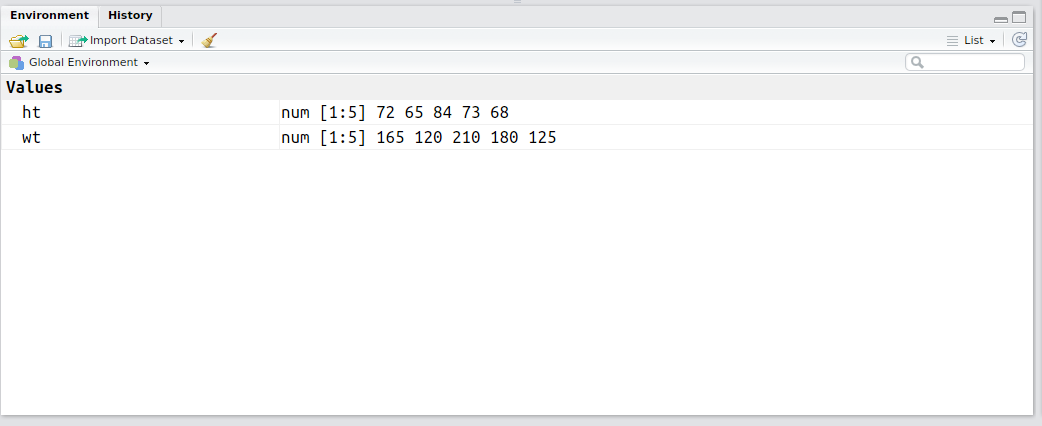
\includegraphics[width = 0.5\textwidth]{figs/environment.png}
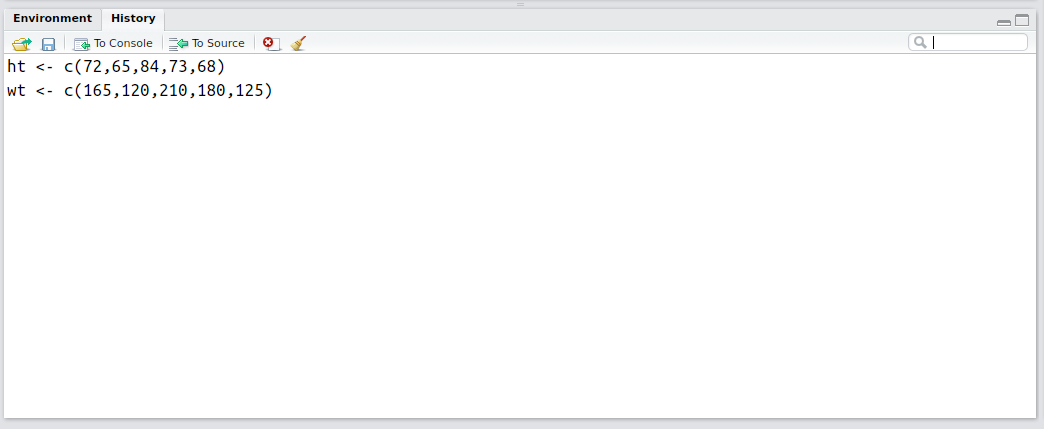
\includegraphics[width = 0.5\textwidth]{figs/history.png} 
\end{frame}

\subsubsection{The file viewer}
\myframe{RStudio: files, plot viewer, packages, help}
The final pane shows us a variety of files/plots: \pause
\begin{spaceitemize}
\item files in the \textcolor{blue}{current working directory} \pause
\item plots generated from executed commands \pause
\item loaded \textcolor{green}{packages} \pause
\item \textcolor{cyan}{help files} that we access \pause
\end{spaceitemize}

We will cover packages and help files later on. 
\end{frame}

\myframe{The working directory}
Folders on your computer are also known as \textcolor{cyan}{directories}. These can contain data, documents, and subdirectories, among many other objects. \pause

Your computer has a home directory, where all of your files (as the user) are stored, in different directories (e.g., \texttt{Documents}, \texttt{Pictures}, etc.). When you first log into your computer, you are in this directory. \pause

The \textcolor{blue}{current working directory} is the directory where you are currently working. To be a bit less obtuse, consider the following example: \pause

You have a file called \texttt{ht\_wt\_analysis.R}, located in the \texttt{Epi-Biost-Workshop} directory, which is a subdirectory of \texttt{UW}, which is a subdirectory of \texttt{Documents}, which is part of your home directory. If you double-click \texttt{ht\_wt\_analysis.R}, which opens RStudio to edit the document, your current working directory is \texttt{<your home>/Documents/UW/Epi-Biost-Workshop}.
\end{frame}

\myframe{Changing the working directory using RStudio}
Generally, when you open RStudio, your current working directory will be your home directory. This can make loading data that you have saved on your computer somewhat difficult. \pause

One way to remedy this is to manually set your working directory using R/RStudio: either \pause
\begin{itemize}
\item Using buttons: \pause
\begin{enumerate}
\item In the file viewer, navigate to the folder where your dataset resides \pause
\item Click on the \texttt{More} button (with the settings-type wheel next to it) under the file viewer tab \pause
\item Click \texttt{Set as working directory} 
\end{enumerate} \pause
\item Using code: \pause
\begin{enumerate}
\item Find the path to the folder where your data resides (e.g., \texttt{/home/brian/Documents/UW/Epi-Biost-Workshop}) \pause
\item Place the code \texttt{setwd("<path to your data>")} in your R script, or enter it at the command line 
\end{enumerate}
\end{itemize}
\end{frame}


\section{Introduction to R programming}
\myframe{Introduction to R programming}
We have already seen some examples of R programming: in the heights and weights example, we learned about the special \texttt{<-} command, which assigns a value to an object; and we learned about the \texttt{c()} command, which creates a vector.  \pause

These commands relate \textcolor{blue}{functions} to \textcolor{green}{objects} -- both of these are fundamental concepts in R programming.
\end{frame}

\myframe{Functions}
R functions take in \textcolor{blue}{arguments} and return \textcolor{green}{values}. A function is accessed by typing its name, followed by an open and closed set of parentheses: e.g., \texttt{quantile()}, a function to compute desired sample quantiles (e.g., minimum, median, maximum). \pause

\textcolor{blue}{Arguments} to functions go between the parentheses, and are separated by columns. You specify which object corresponds to which argument using \texttt{=}, e.g., \texttt{quantile(x = ht, probs = 0.5)} returns the median value of the \texttt{ht} object. \pause 

\textcolor{green}{Values} are returned by functions, and are generally either a combination of objects, plots, and printout. The value of the result of entering \texttt{quantile(x = ht, probs = 0.5)} into the console is a vector containing the number 72.
\end{frame}

\myframe{Objects}
R objects are (basically) the result of calling functions. However, there are two general ways this can be done: \pause
\begin{spaceitemize}
\item \textcolor{blue}{loading data} (e.g., from a text or .csv file) \pause
\item \textcolor{green}{manipulating another object} using a function \pause
\end{spaceitemize}

Both \texttt{ht} and \texttt{wt} are objects; we created them by manipulating raw numbers using the \texttt{c()} function.
\end{frame}

% Accessing and manipulating data
\section{Accessing and manipulating data}
\myframe{Loading data}
Data can be loaded using \textcolor{blue}{menus}, \textcolor{green}{buttons}, or a \textcolor{cyan}{function}.  \pause

The menus and buttons ultimately call a function; each data storage type (e.g., \texttt{.txt}, \texttt{.csv}, \texttt{.sas7bdat}, \texttt{.dta}) has its own function (and some functions come from special packages). \pause

Regardless of how you load the data, once done it will show up in your environment. It can then be manipulated to display summary statistics, make plots, or do more complex analyses.
\end{frame}

\myframe{Loading data: menus}
\begin{enumerate}
\item Go to \texttt{File > Import Dataset} \pause
\item Select the type of data from the menu (e.g., \texttt{From CSV}) \pause
\item Browse to the directory or website where the data are stored \pause
\item Specify any input options \pause
\item Edit the \texttt{Code Preview} section to rename the object, if necessary \pause
\item Click \texttt{Import}
\end{enumerate}

\end{frame}

\myframe{Loading data: buttons}
\begin{enumerate}
\item In the \texttt{Environment} pane, click \texttt{Import Dataset} \pause
\item Select the type of data from the menu (e.g., \texttt{From CSV}) \pause
\item Browse to the directory or website where the data are stored \pause
\item Specify any input options \pause
\item Edit the \texttt{Code Preview} section to rename the object, if necessary \pause
\item Click \texttt{Import} 
\end{enumerate}
\end{frame}

\myframe{Loading data: menus and buttons}
Regardless of whether you use a menu or button to import data, there was a step where you had to look at the \texttt{Code Preview} box. When you click the \texttt{Import} button, this code is executed in the console, and the dataset shows up in your environment. \pause

This means that, under the hood, \textcolor{blue}{both methods use R code to import data}! 

Also, both of these methods are \textcolor{red}{hard to reproduce}: each time you want to analyze a dataset (which may be multiple times on a problem set or during the course of a project/paper), you have to click through these buttons. \pause

To make your code fully reproducible, \textcolor{cyan}{embed the code} to load the data \textcolor{cyan}{directly in your R script}! While this involves finding the correct functions, at the end of the day you have more control over how your data are handled.
\end{frame}

\myframe{Loading data: functions}
\begin{enumerate}
\item Find the path to your data file \pause
\begin{itemize}
\item {\scriptsize e.g., \texttt{"/home/brian/Documents/UW/Epi-Biost-Workshop/ht\_wt\_data.txt"} }
\end{itemize}
\item Based on the file extension (e.g., \texttt{.txt}, \texttt{.csv}, \texttt{.dta}), choose the appropriate function \pause
\item Put the function call with the file path in your R script with the desired options \pause
\begin{itemize}
\item {\tiny e.g., \texttt{read.table("/home/brian/Documents/UW/Epi-Biost-Workshop/ht\_wt\_data.txt", sep = "", header = TRUE)} } \pause
\end{itemize}
\item Run this line to load the data
\end{enumerate}
\end{frame}

\myframe{Loading data: common functions and packages}
\begin{tabular}{rrr}
File extension & Package & Function \\
\hline 
\texttt{.txt} & \texttt{utils} (always loaded)  & \texttt{read.table()} \\
              &                & \texttt{read.delim()} \\
              & \href{http://readr.tidyverse.org/}{\texttt{readr}} & \texttt{read\_table()} \\
              &                & \texttt{read\_delim()} \\
\texttt{.csv} & \texttt{utils}  & \texttt{read.csv()} \\
              & \texttt{readr} & \texttt{read\_csv()} \\
\texttt{.dta} & \href{http://haven.tidyverse.org/}{\texttt{haven}} & \texttt{read\_stata()} \\
\texttt{.sas7bdat} & \texttt{haven} & \texttt{read\_sas()} \\
\texttt{.xlsx} & \href{http://readxl.tidyverse.org/}{\texttt{readxl}} & \texttt{read\_excel()} \\
\texttt{.Rdata} & \texttt{base} (always loaded) & \texttt{load()} \\
\texttt{.Rds} & \texttt{base} & \texttt{readRDS()} \\
\hline
\end{tabular}
\end{frame}

\begin{frame}[fragile]
\frametitle{Exercise: Reading in data}

Load the height and weight data by placing the following code in your R script \texttt{ht\_wt\_analysis.R} (replace \texttt{<path to here>} with the path to your folder):

{\small
\begin{verbatim}
dat <- read.table("<path to here>/Epi-Biost-Workshop/
                  day_3_session_1/data/ht_wt_data.txt",
                   header = TRUE)
\end{verbatim}
}

Look at the data by typing \texttt{View(dat)} on a new line in your R script, and executing the line in R. 

What do you notice about this new dataset? How does it relate to the two vectors \texttt{ht} and \texttt{wt} that we created earlier?
\end{frame}

\begin{frame}
\frametitle{Exercise: reading data}
Now read in the FEV data, again using the function \texttt{read.table}. \textit{Hint: you may copy the code from the height and weight example, but you will have to change the path to the data}.

Again, use the \texttt{View()} function to take a look at the data, and answer the following questions:
\begin{enumerate}
\item How many columns do the data have?
\item Write down what you think the meaning of at least 3 of the variables is, based on the column names.
\end{enumerate}  
\end{frame}

\myframe{Manipulating data}
A large component of any data analysis is getting the data into a useable format for our analysis: this usually involves a combination of creating new variables and taking subsets of the data. \pause

The two most common types of data you will see are \textcolor{green}{vectors} \pause and \textcolor{blue}{data frames}. \pause We have already been introduced to vectors in the heights and weights example; \pause data frames are generally datasets, where the columns are \textcolor{cyan}{variables} (each of these is a vector), and the rows are \textcolor{purple}{observations}. \pause

By manipulating the columns of a data frame we create new variables or change existing ones; and by manipulating the rows of our data we restrict our attention to different subsets of the observations.
\end{frame}

\myframe{Manipulating data: accessing values in vectors}
The easiest way to access data is from a vector: each vector is its own variable, and hence we just need to extract the correct element(s). \pause

To access the $i$th element in the vector \texttt{vec}, we use square brackets; \texttt{vec[i]} accomplishes this. For example, \texttt{ht[1]} returns the first element in the \texttt{ht} vector, which is the height of our first imaginary individual. \pause

To access a continuous range of elements $i$ through $l$, use square brackets with a colon; \texttt{vec[i:l]} accomplishes this. For example, \texttt{ht[1:4]} returns the first four elements of \texttt{ht}. \pause

To access a set of elements ($i$, $k$, $n$), use square brackets with \texttt{c()}; \texttt{vec[c(i, k, n)]} accomplishes this. For example, \texttt{ht[c(1, 3, 5)]} returns the first, third, and fifth elements of \texttt{ht}.
\end{frame}

\myframe{Manipulating data: accessing values in data frames}
Data frames have both rows and columns. The dimensions of the data frame are first rows, then columns. \pause We can access a single value in a data frame by first specifying the desired row, then the desired column, within square brackets; \pause for a data frame \texttt{dat} with 5 rows and 2 columns, we can get the first observation from the second column using \texttt{dat[1, 2]}. \pause

For example, in the heights and weights data, \texttt{dat[1, 2]} returns the weight of the first individual. \pause

We can use the same rules as those for vectors to select groups of rows and/or columns. 
\end{frame}

\myframe{Manipulating data: accessing variables in data frames}

There are three ways to access a variable in a data frame. For a data frame \texttt{dat}, with columns \texttt{x} and \texttt{y}, we can use: \pause
\begin{spaceitemize}
\item \texttt{\$}; \texttt{dat\$y} returns the variable \texttt{y} from the data frame \texttt{dat} \pause
\item the column number; \texttt{dat[, 2]} returns the variable \texttt{y} from \texttt{dat} \pause
\item the column name; \texttt{dat[, "y"]} returns the variable \texttt{y} from \texttt{dat}
\end{spaceitemize} \pause

The methods using the square brackets introduce a new concept: we are selecting \textcolor{purple}{all rows} from \texttt{dat} (since there is nothing between the first bracket and the comma), and are selecting \textcolor{blue}{certain columns} from \texttt{dat}. 
\end{frame}

\myframe{Manipulating data: subsetting data frames}
Often, we don't know exactly which rows we want to select. Using \textcolor{blue}{logical} operations helps us select participants with certain characteristics. Logical operations return \texttt{TRUE} or \texttt{FALSE}. \pause

The common logical operations are:
\begin{tabular}{rrr}
Operation & Meaning & Result \\
\hline 
\texttt{|} & or & \texttt{TRUE} if any argument is \texttt{TRUE} \\
\texttt{\&} & and & \texttt{TRUE} only if all arguments are \texttt{TRUE} \\
\texttt{!} & negation & \texttt{FALSE} if argument returns \texttt{TRUE}, \texttt{TRUE} else \\
\texttt{==} & equals & \texttt{TRUE} if the two arguments are equal \\
\hline
\end{tabular}

We can also make comparisons, using \textless, \textgreater, \textless =, \textgreater =.
\end{frame}

\begin{frame}[fragile]
\frametitle{Example: heights and weights}
The following code loads the data as a data frame, and then: prints out the height column, and displays the data from participants whose weight is below 160 lbs (replace \texttt{<path to here>} with your own path):
{\scriptsize
\begin{verbatim}
## load using read.table
dat <- read.table("<path to here>/Epi-Biost-Workshop/
                  day_3_session_1/data/ht_wt_data.txt", header = TRUE)
## print out the height column multiple ways
dat$height
dat[, "height"]
dat[, 2]

## print out the observations with weight under 160
dat[dat$weight < 160, ]

\end{verbatim}
}
\end{frame}

\begin{frame}
\frametitle{Exercise: manipulating data}
These questions all pertain to the \texttt{fev} data. 

\begin{enumerate}
\item The logical expression \texttt{fev\$age <= 8} returns \texttt{TRUE} for those individuals who are less than or equal to 8 years old, and \texttt{FALSE} for those who are older than 8 years old. Create a new dataset called \texttt{sub\_less\_equal\_8} that contains the data for all participants with age less than or equal to 8 years old.
\item What does \texttt{fev\$sex == 1} return?
\item The \texttt{\$} allows you to both access variables and create new variables within a dataset. Create a new variable called \texttt{fev\$female} that takes value 0 if the participant is male and 1 if the participant is female, using the command \texttt{fev\$female <- ifelse(fev\$sex == 1, 0, 1)}. What is the sex of the participant with \texttt{fev\$subjid == 451}?
\end{enumerate}
\end{frame}

\section{Summarizing data}
\begin{frame}
\frametitle{Summarizing data}
The first part of my data analysis workflow (after reading in the data) is typically \textbf{exploratory}. Here, I investigate whether I can find any trends in the data that support my initial hypothesis. \pause

Two powerful ways of summarizing the data are:\vspace{-0.3cm} \pause 
\begin{itemize}
\item summary statistics (e.g., mean, median) \pause
\item graphical summaries (e.g., boxplots, scatterplots)
\end{itemize}
\end{frame}


\begin{frame}[fragile]
\frametitle{Computing summary statistics}
Quick summary statistics are available in R using the \texttt{summary()} function. This function automatically computes the minimum, mean, maximum, and 25th, 50th (median) and 75th percentile values of \textcolor{blue}{each variable} in your data.

Example: heights and weights
\begin{verbatim}
summary(dat)
\end{verbatim}
\end{frame}

\begin{frame}[fragile]
\frametitle{Plotting data}
Quick plots are also powerful ways to convey information and get a glimpse at trends in the data.

The most common type of plot that I use is a scatterplot. You create a scatterplot using the \texttt{plot()} function. \pause

The two main arguments, \texttt{x} and \texttt{y}, tell R the data to plot on the x- and y-axis, respectively. Other arguments help to make the plot understandable by adding informative labels and titles.

Example: heights and weights
\begin{verbatim}
# plot of height (on x-axis) vs weight
plot(dat$height, dat$weight)
\end{verbatim}
\end{frame}

\begin{frame}
\frametitle{Exercise: summarizing data}
All of these questions involve either the full \texttt{fev} data, or the subset of participants with age less than or equal to eight years old \texttt{sub\_less\_equal\_8}.

\begin{enumerate}
\item What is the average age of participants in the \texttt{fev} data?
\item What is the proportion of subjects that are female? That are male?
\item What is the average FEV measurement in the full data?
\item What is the average FEV measurement in those who are less than or equal to eight years old?
\item If your answers to 3 and 4 are different, why do you think that is?
\item Plot FEV on the y-axis versus age on the x-axis for the full data. What do you notice about the trend between age and FEV? Does that help you answer 5?
\end{enumerate}
\end{frame}

\section{R packages}
\myframe{R packages}
Functions in R are available through \textcolor{blue}{packages}. Each package contains a specific set of functions, and must be both \textcolor{green}{installed} and \textcolor{cyan}{loaded} before the function can be used. \pause

Each package only has to be \textcolor{green}{installed once}, \textcolor{purple}{unless you upgrade your version of R}. Packages are installed using the \texttt{install.packages()} function. \pause

Each time you open a new R session, \textcolor{cyan}{you have to re-load} all R packages you wish to use in the session. Packages are loaded using the \texttt{library()} function. \pause

However, some packages are always loaded each time you open R. These are \texttt{stats}, \texttt{graphics}, \texttt{grDevices}, \texttt{utils}, \texttt{datasets}, \texttt{methods}, and \texttt{base}.
\end{frame}

\myframe{Finding new R packages}
In general, R packages are stored on one (or more) of three \textcolor{blue}{repositories}: \pause \href{https://cran.r-project.org/}{CRAN}, under the \texttt{Packages} side-menu; \pause \href{https://www.bioconductor.org/}{Bioconductor}, under the \texttt{Explore packages} menu; \pause and individual programmer's GitHub pages (e.g., the repository for the \href{https://github.com/hadley/devtools}{\texttt{devtools} package}, for easy R package creation). \pause

You can install packages from CRAN using \texttt{install.packages()}; \pause from Bioconductor by first running \texttt{source("https://bioconductor.org/biocLite.R")} and then using \texttt{biocLite()}; \pause and from GitHub using the function \texttt{install\_github()} from the \texttt{devtools} package.
\end{frame}

\begin{frame}[fragile]
\frametitle{Example: heights and weights}
The following code reads in the height and weight data using the \texttt{read\_table()} function from \texttt{readr}:
{\scriptsize
\begin{verbatim}
## install if necessary
# install.packages("readr")
## load the package; do this each time you re-open R!
library("readr")
## read in the data
dat <- read_table("<path to here>/Epi-Biost-Workshop/
                   day_3_session_1/ht_wt_data.txt", header = TRUE)
\end{verbatim}
}
\end{frame}

\end{document}